

\chapter{Solução de suprimento de energia}
Considerando que o sistema radar possui o funcionamento em regime permanente, o dimensionamento da fonte de alimentação para o produto comercial foi realizado considerando os consumos energéticos da iluminação e dos componentes eletrônicos. Porém, devido às limitações de orçamento e recursos disponíveis, o dimensionamento do protótipo a ser construído foi realizado considerando o funcionamento do radar durante 1/4 do dia,para a alimentação das cargas mostradas na Figura \ref{fig30}.

\begin{figure}[h!]
\centering \label{fig30}
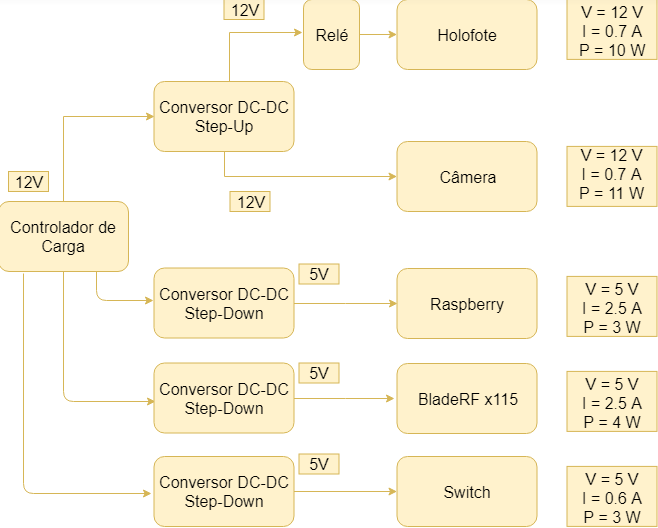
\includegraphics[scale=0.5]{pot}
\caption{Diagrama de alimentação de energia pela geração fotovoltaica }
\label{fig:circ}
\end{figure}

A Figura acima representa as cargas que devem ser alimentadas pela geração fotovoltaica assim como os conversores adotados para garantir que chegue a tensão correta para as cargas. O conversor Step-up vai garantir que chegue os 12V nas cargas que necessitam de 12V e o conversor Step-down vai diminuir o valor da tensão para 5V para as cargas que precisam de apenas 5V, funcionando como uma proteção as cargas.

A Figura \ref{fig31} representa a integração entre o escopo da engenharia de energia e a engenharia eletrônica dentro do projeto do radar. Os itens em amarelo representa o escopo de energia e os itens em azul representa o escopo de eletrônica.

\begin{figure}[h!]
\centering \label{fig31}
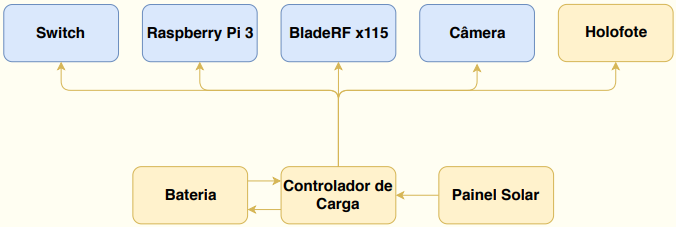
\includegraphics[scale=0.6]{energronica}
\caption{Diagrama de integração energia-eletrônica }
\label{fig:circ}
\end{figure}

\section{Recurso Solar}

O projeto será instalado e testado inicialmente no Campus FGA da Universidade de Brasília, localizado no Gama, cujas as coordenadas são: 15º59’24”S e 49º02’43”.A partir das coordenadas, é possível verificar os valores de irradiação solar diária média do local mais próximo na base de dados do CRESESB.
O radar tem a ideia de ser instalado em todas as regiões serranas do Brasil, com isso recomenda-se um estudo de caso sobre a irradiação solar diária em cada região que o radar for implantado, para se obter um melhor rendimento solar do sistema fotovoltaico implantado. 
\begin{figure}[h!]
\centering
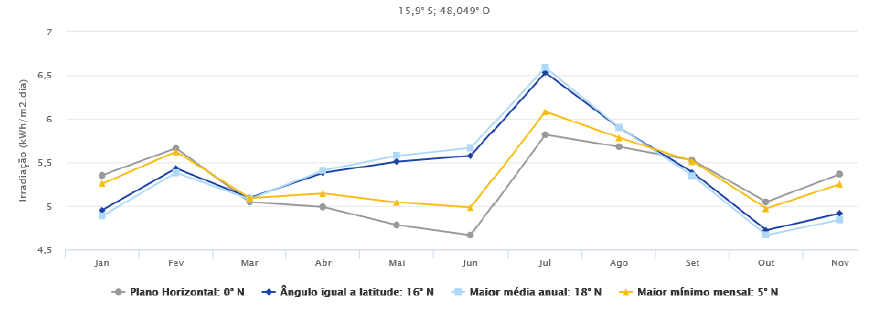
\includegraphics[scale=0.5]{grafico}
\caption{Irradiação Solar Gama-Brasília-DF}
Fonte: CRESESB
\label{fig:grafico}
\end{figure}

\begin{figure}[h!]
\centering
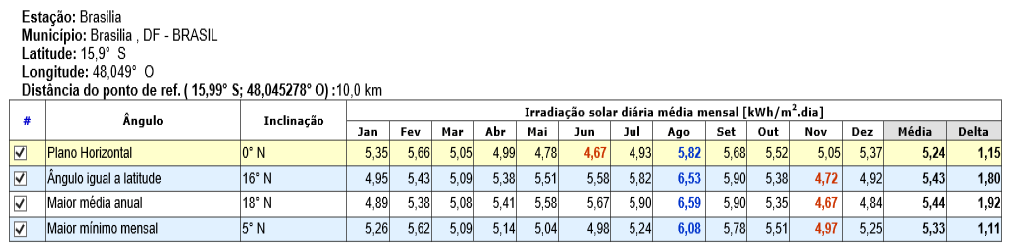
\includegraphics[scale=0.5]{tabela}
\caption{Valores de irradiação solar média}
Fonte: CRESESB
\label{fig:tabela}
\end{figure}

Verifica-se na tabela que a maior média anual de Brasília é de 5,44 $KWh/m^2dia$, que é um ótimo valor comparado a outras regiões. Aliado á baixa nebulosidade e pluviosidade, o Distrito Federal é um local ideal para implantação de sistemas fotovoltaicos.

\subsubsection{Definição da inclinação do painel}

 A inclinação dos módulos fotovoltaicos instalados é determinado de acordo com a latitude do local. A localização em questão possui os dados de latitude iguais a $15^{\circ}59’24”$ S. Analisando então os dados de irradiação solar fornecidos pelo Centro de Referência em Energia Solar e Eólica - CRESESB, temos que, na região de Brasília, o ângulo considerado é o ângulo de $15^{\circ}$. Dessa forma, devido á proximidade dos ângulos e os dados obtidos, será utilizado neste projeto o ângulo de inclinação de 15º para o módulo fotovoltaico.
 Com isso, de acordo com a tabela 1 será considerado para os  cálculos os dados que  trata da radiação global no plano inclinado  igual á latitude para a localidade.
 
\section{Dimensionamento da Placa Fotovoltaica}

O dimensionamento do painel fotovoltaico levou em consideração o suprimento de toda a carga do sistema radar, como mostra a Tabela \ref{tab24}, que representa a carga a ser alimentada pela geração fotovoltaica. 

\begin{table}[H]
\caption{Cargas a serem alimentadas pela geração solar}\label{tab24}
\begin{tabular}{|c|c|c|c|}
\hline
\multicolumn{4}{|c|}{Consumo de energia durante 24 horas de funcionamento do radar}                                                 \\ \hline
Dispositivos & Potência & Tempo de consumo diário & Consumo total diário \\ \hline
Raspberry Pi 3  & 30W  & 24  & 720W  \\ \hline
Câmera & 8.4W  & 12 & 100.8W \\ \hline
BladeRFmx115 & 30W  & 24 & 720W \\ \hline
LED       & 8.4W &  12 & 100.8W  \\ \hline
Switch       & 8.4W &  12 & 100.8W \\ \hline
Total & 84W & - & 1814.4W \\ \hline

\end{tabular}
\end{table}
\FloatBarrier

Considerando o funcionamento do radar em um período de 24 horas e que necessariamente a BladeRF, Raspberry e Switch precisariam funcionar durante as 24 horas e apenas a iluminação e a câmera funcionaria em um período médio de 12 horas. O consumo total da carga é 1814,4 Wh e a potência mínima dos painéis de geração séria 480,51 Wp.

A Tabela \ref{tab6} apresenta o consumo das cargas durante um período de 6 horas.

\begin{table}[H]
\begin{tabular}{|c|c|c|c|} \label{tab6}


Dispositivos             & Potência         & Tempo de consumo diário & Consumo total diário \\ \hline
Raspberry Pi 3  & 30W  & 6 horas          & 180W    \\ \hline
Câmera & 8.4W  &   3 horas        & 25.2W \\ \hline
BladeRFmx115 & 30W  & 6 horas         & 180W \\ \hline
LED       & 8.4W &  3 horas & 25.2W    \\ \hline
Switch       & 8.4W &  6 horas & 50.4 W    \\ \hline
Total & 84W & - & 460.8 W \\ \hline

\end{tabular}
\end{table}
\FloatBarrier

Para este trabalho será considerado para os cálculos e compra de materiais uma autonomia de 6 horas para o funcionamento do radar. Com isso para a BladeRf, Raspberry e Switch será considerado a autonomia total de 6 horas e para a iluminação e câmera será considerado 3 horas. Com essas considerações temos uma necessidade de suprir uma carga de 453,8 Wh e uma potência mínima de:
\begin{equation}
    Pmin = \frac{Potencia total}{(HSP)(FS)} 
\end{equation}
\begin{equation}
    \frac{453,8}{(4,72)(0,8)} = 120,18 Wp
\end{equation}
onde, 

HPS = horas de sol pleno

FS = rendimento dos componentes, bateria, controlador e perdas nos fios.

A variável HSP é determinada por meio do valor da radiação do mês que apresentou o menor índice, este valor pode ser observado na figura apresentada com os dados do CRESESB na irradiação global no plano inclinado igual á latitude para a localidade. A menor radiação observada para a localidade foi no mês de novembro no valor de 4,72 $kWh/m^2dia$. 
 
De acordo com os cálculos acima a potência miníma dos painéis a ser instalada no período de suprimento citado será de 120,18 Wp. Há a possibilidade de conseguirmos o fornecimento de quatro painéis de 50Wp, sendo viável ao projeto devido ao elevado custo. O excesso de potência dos quatro painéis seria bom, pois a carga final não está fechada nas outras áreas que envolve a construção do radar podendo assim aumentar. 

Os quatro painéis vão ser conectados em paralelo com o objetivo de aumentar a tensão para ser o suficiente para a alimentação das cargas, que precisam de no mínimo 7A de corrente. 

\begin{figure}[h!]
\centering
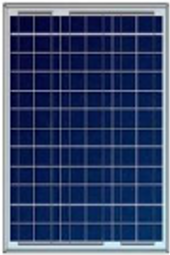
\includegraphics[scale=0.6]{placa}
\caption{Representação do painel fotovoltaico 50W}
Fonte: Komaes 50W
\label{fig:tabela}
\end{figure}

\section{Dimensionamento da Bateria}
Componente fundamental do sistema autônomo, pois como o nome já disse, ele precisa ser totalmente independente de qualquer outra fonte primária de energia elétrica e a escolha adequada da capacidade da bateria é de muita importância, pois ela garante a continuidade do fornecimento da energia elétrica mesmo em condições adversas para a geração fotovoltaica, exemplificando, durante o período noturno e nos dias de chuva \cite{alan}.
\begin{itemize}
 \item\textbf{Dimensionamento do produto comercial}
\end{itemize}
Levando em consideração a carga total do sistema 84W e considerando dias nublados e períodos em que não há irradiação, a bateria deve ser capaz de alimentar o sistema por 24 horas.
Então, a energia diária consumida é realizada com base no consumo diário de cada dispositivo e já considerado seu dispositivo de proteção, apresentado na Tabela \ref{tab24}.

Com os valore obsersados na Tabela \ref{tab24}, é possível calcular a capacidade do sistema de acumulação a partir das equações \cite{alan}:

\begin{equation}
    C_{Bat} = \frac{CB*N}{Pd*Ef}\\
\end{equation}




Sendo,

\textbf{CBat}: Capacidade total da bateria;

\textbf{CB}: energia diária solicitada pelas cargas por dia em Ah;

\textbf{N}: número de dias de autonomia;

\textbf{Pd}: máxima profundidade de descarga da bateria (tipicamente varia de 50 a 80\%);

\textbf{Ef}: eficiência da bateria;

Sendo 12 volts a tensão padrão das baterias comerciais, obtemos o valor de consumo diário de 151.2 Ah. Fixando-se um valor de N igual a 1 dia e um valor de Pd igual a 70\% e o valor da eficiência como 90\% obtém-se os valores de capacidade de:

\begin{equation}
    C_{Bat} = \frac{151.2*1}{0.7*0.9}\\
\end{equation}

\begin{equation}
    CB = 240 Ah
\end{equation}



Dessa forma, optou-se por uma bateria de 12V da marca Heliar Freedom com uma capacidade de 185Ah associada em paralelo com outra bateria da mesma marca com capacidade de 70Ah.Na Figura \ref{fig:bateria185} e \ref{fig:bateria70} serão apresentadas a bateria escolhidas por possuirem os melhores parâmetros de preço e qualidade.

\begin{figure}[h!]
\centering
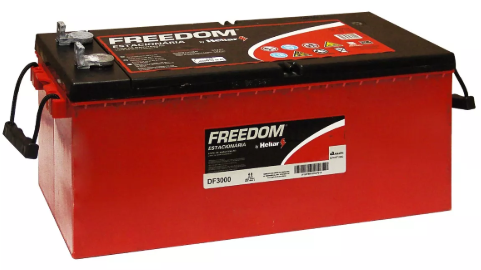
\includegraphics[scale=0.4]{bateria185}
\caption{Bateria Heliar Freedom de 185Ah escolhida para o Sistema de Armazenamento}. Fonte: %\cite{bateria_heliar_115}.
\label{fig:bateria185}
\end{figure}
\pagebreak

\begin{figure}[h!]
\centering
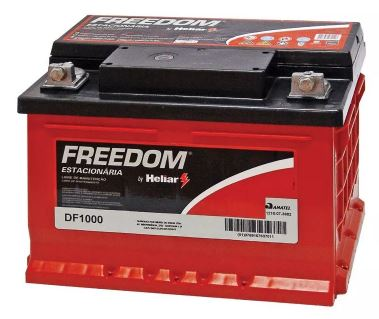
\includegraphics[scale=0.4]{bateria70}
\caption{Bateria Heliar Freedom de 70Ah escolhida para o Sistema de Armazenamento}. Fonte: %\cite{bateria_heliar_70}.
\label{fig:bateria70}
\end{figure}

    \begin{itemize}
        \item \textbf{Dimensionamento do protótipo}
    \end{itemize}
    
    De maneira análoga, é feito o dimensionamento da bateria considerando 6 horas de funcionamento do radar por dia, devido ao orçamento restrito e os recursos disponíveis. A Tabela \ref{tab6} apresenta o consumo diário de potência do sistema radar com seu funcionamento durante 6 horas por dia.
    
\begin{equation}
    C_{Bat} = \frac{38.4*1}{0.7*0.9}\\
\end{equation}

\begin{equation}
    CB = 60.95 Ah
\end{equation}


Dessa forma, optou-se por uma bateria de 12V da marca Heliar Freedom com uma capacidade de 70Ah. Na Figura \ref{fig:bateria71} será apresentada a bateria escolhida por possuir o melhor parâmetro de preço e qualidade.


\begin{figure}[H]
\centering
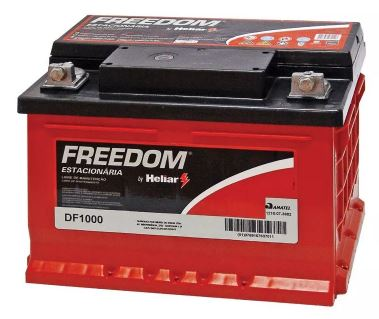
\includegraphics[scale=0.4]{bateria71}
\caption{Bateria Heliar Freedom de 70Ah escolhida para o Sistema de Armazenamento}. Fonte: %\cite{bateria_heliar_70}.
\label{fig:bateria71}
\end{figure}
\FloatBarrier

\section{Dimensionamento do Controlador de Carga}

Para o correto dimensionamento do controlador de carga é preciso conhecer as máximas correntes às quais ele será submetido, tanto do lado dos painéis geradores quanto do lado das cargas. A corrente máxima, circula no lado dos painéis geradores e possui valor de 15,75 A. Portanto, foi selecionado o controlador de carga da marca Charge Controller com limite de carga e descarga de 20A.Na Figura \ref{fig:control}, será apresentado o controlador de carga escolhido.

\begin{figure}[H]
\centering
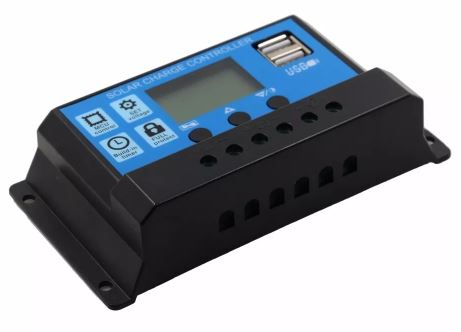
\includegraphics[scale=0.4]{control}
    \caption{Controlador de carga da marca Charge Controller com limite de 10A escolhida para o Sistema de Proteção}. Fonte:\cite{controlador}.
\label{fig:control}
\end{figure}
\FloatBarrier

\section{Dimensionamento da Iluminação}

Com o objetivo de alertar o motorista quando houver outro veículo em sentido contrário, a solução para o subsistema iluminação foi: cada totem terá um holofote com lâmpada LED da marca SR,onde a fonte de alimentação é um barramento infinito alimentado pela bateria, onde a energia é transferida do barramento para a luminária através de um condutor conectado com um relé. 

Tendo em vista o custo-benefício, foi escolhido para a iluminação um holofote LED com função RGBW para o subsistema iluminação. Na Figura \ref{fig:holofotergbw} será apresentada a luminária escolhida.

    \begin{figure}[h!]
\centering
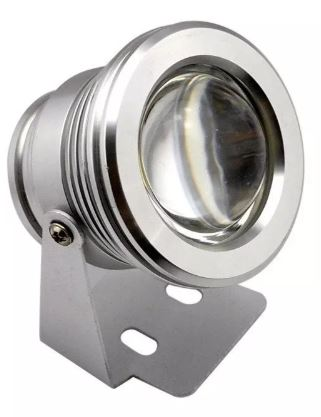
\includegraphics[scale=0.3]{holofotergbw}
\caption{Lúminária LED RGBW}. Fonte: \cite{holofote}.
\label{fig:holofotergbw}
\end{figure}
\vspace*{\fill}
\pagebreak

Na Tabela \ref{tab:luminaria} serão apresentados os dados técnicos da luminária escolhida.
    \begin{table}[H]
    \label{tab:luminaria}

\begin{tabular}{|c|c|c|c|c|c|c|}
\hline
\multicolumn{7}{|c|}{Dados da luminária escolhida}                                                 \\ \hline
Marca             & Tensão         & Corrente & Potência & Altura & Largura & Comprimento \\ \hline
Panabraks Comercial  & 12V  & 0.83          & 10W   & 10.3cm & 7.2cm & 7.2cm \\ \hline

\end{tabular}
    \caption{Tabela de dados da luminária}
\end{table}
\FloatBarrier

\section{Dimensionamento dos dispositivos de proteção}

\begin{itemize}
    \item \textbf{Conversor DC-DC}
\end{itemize}
O conversor DC/DC  é um conversor de tensão que converte um nível de tensão inicial em outro secundário, regulando a tensão de saída em relação a uma tensão de entrada. Foi escolhido por causa da alta eficiência (perda típica de 12\% da potência de entrada) para fornecer a tensão que os componentes eletrônicos demandam. No projeto serão utilizados três conversores step-down e um conversor step-up.
    
Seu circuito é composto por uma chave (S), a qual permanece fechada por um tempo t.on e aberta por um tempo t.off, durante um tempo de chaveamento T. A chave está ligada a um filtro composto por um indutor (L) e um capacitor (C) , que têm a função de uniformizar os parâmetros de tensão que chegam à carga. Ocorre que, a chave não pode ser aberta se a corrente que passa por ela não for nula, pois causaria uma sobretensão no indutor. Com isso, utiliza-se um diodo de retorno (D), que proporciona um caminho para a corrente do indutor (iL) enquanto a chave estiver aberta. Na Figura \ref{fig:circuitostepdown} será apresentado o circuito do conversor DC-DC \cite{Amauri}.

\begin{figure}[H]
\centering
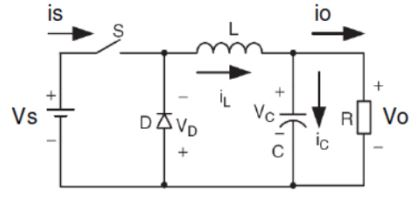
\includegraphics[scale=0.9]{circuitostepdown}
    \caption{Circuito elétrico do Conversor DC-DC.}. Fonte: \cite{Amauri}.
\label{fig:circuitostepdown}
\end{figure}
\FloatBarrier

Para dimensionar o conversor DC-DC adequado para a Raspberry e a BladeRFx115, dimensionamos a partir da tensão de entrada dos módulos, que tem como fonte a bateria de 12 volts a necessidade de uma tensão de saída (Vo) de 5V. Como a corrente que circulará na Raspberry e na BladeRFx115  é 2,5 A, o valor da resistência para cada conversor DC-DC será igual a: 5=R*2,5 sendo R= 2 ohm. \cite{MSM}.

Para dimensionar o conversor do circuito do Switch, possuímos a mesma tensão de entrada e saída. Porém, a corrente que circula nessa carga é de 0,6 A. Logo, o valor da resistência será igual a 5=R*0.7 sendo R= 7,14 ohm.

Para o circuito da câmera e do holofote, a tensão de entrada também corresponde a tensão da bateria, de 12 volts e a tensão de saída (Vo) é 12.5 volts. Como a corrente que circulará no circuito em paralelo do holofote e da câmera é 1,4 A, o valor da resistência para cada conversor DC-DC será igual a: 12,5=R*1,4 sendo R= 8,92 ohm.

Os Conversores DC/DC utilizados no circuito da Raspberry, BladeRFx115, Switch, Holofote e Câmera são do modelo XL6019, suportam tensões de entrada de 6 a 40VDC, e consegue fornecer, de forma ajustável, uma tensão de 1,3 a 35 V e uma corrente de até 5A, tendo um rendimento de 94\%.Na Figura \ref{fig:conversordc} será apresentado o Conversor DC-DC escolhido para o projeto.

\begin{figure}[H]
\centering
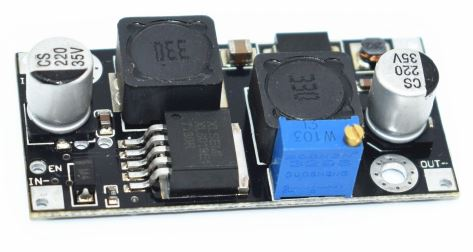
\includegraphics[scale=0.6]{conversordc}
    \caption{Conversor DC-DC modelo XL6019 escolhido para o sistema de proteção das cargas}. Fonte: \cite{conversor}.
\label{fig:conversordc}
\end{figure}
\FloatBarrier


\begin{itemize}

    \item \textbf{Relé}
    
\end{itemize}

O relé é um interruptor eletromecânico, se movimenta fisicamente com a passagem de corrente elétrica pelas espiras de sua bobina, criando assim um campo eletromagnético que atrai a alavanca responsável pela mudança do estado entre os contatos. Além disso, sabe-se que para energizar corretamente um relé, e ativar suas chaves internas, é necessário que uma corrente de intensidade mínima circule pela sua bobina. Sendo assim, deve-se aplicar uma tensão de determinado valor, que devido a resistência do enrolamento, permita que essa corrente circule pelos terminais da bobina. Os relés são especificados por sua de tensão nominal na bobina, a corrente máxima da chave e o valor de corrente que deve circular na bobina \cite{Braga}.

Para o projeto, foi escolhido o Módulo Relé 1 canal-5V com corrente típica de operação 15~20mA, com capacidade de 30VDC e 10A e tempo de resposta de 5-10ms. Na figura \ref{fig:rele} será apresentado o relé escolhido para o sistema de proteção do circuito da câmera.

\begin{figure}[H]
\centering
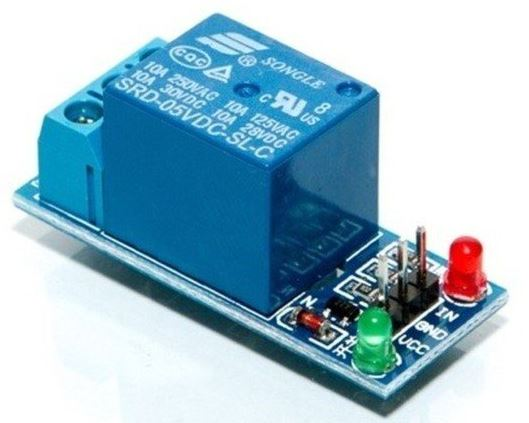
\includegraphics[scale=0.5]{rele}
    \caption{Módulo relé 1 canal-5V escolhido para o circuito de proteção da câmera}. Fonte: \cite{rele}.
\label{fig:rele}
\end{figure}
\FloatBarrier

\subsection{Dimensionamento dos cabos}

A seção transversal do cabo deve ser dimensionada em função da corrente máxima de serviço que atravessa o cabo. De acordo com a norma europeia IEC 60364-7-712 o cabo deve ser capaz de suportar 1,25 vezes a corrente de curto-circuito do gerador e estar protegido contra falhas de terra e curto-circuito. 

Neste projeto, os cabos deverão suportar, I = 7A x 1,25 = 8,75A do controlador de carga e a alimentação de carga.Por possuir quatro painéis ligados em paralelo e cada painel possui Icc = 3,04 A a corrente considerada para o dimensionamento foi I = 12,6A x 1,25 = 15,75 A entre o painel e o  controlador de carga, considerando a corrente de curto circuito do painel. I = 7,3A x 1,25 = 9,12 A entre a bateria e o controlador de carga. Outro ponto importante é a queda de tensão nos cabos que deve ser reduzida com o aumento da bitola, evitando uma queda de tensão significativa.

Considerando a ABNT NBR 5410, o método de instalação B1 e que teremos dois condutores carregados um positivo e um negativo, e que a temperatura pode chegar a 60 graus Celsius. O fator de correção a 60 graus Celsius será 0,50.  Dessa forma, será utilizado um condutor com seção de $4mm^2$ para toda a fiação que a corrente for até 16A (32x0.5 = 16A) e a fiação do painel solar até o controlador de carga será utilizado um condutor de $6mm^2$, consegue suportar a corrente que o painel irá transmitir ao controlador de carga. 

O condutor de proteção será calculado a partir da seção dos condutores de fase do circuito, de acordo com a tabela:

\begin{table}[h]
 \centering
 \caption{Seção miníma dos condutores de proteção}
% distancia entre a linha e o texto
 {\renewcommand\arraystretch{1.25}
 \begin{tabular}{ l l }
  \cline{1-1}\cline{2-2}  
    \multicolumn{1}{|p{4.133cm}|}{Seção miníma dos condutores de fase (mm²) \centering } &
    \multicolumn{1}{p{4.450cm}|}{Seção miníma dos condutores de proteção (mm²) \centering }
  \\  
  \cline{1-1}\cline{2-2}  
    \multicolumn{1}{|p{4.133cm}|}{S\textless = 16 \centering } &
    \multicolumn{1}{p{4.450cm}|}{S \centering }
  \\  
  \cline{1-1}\cline{2-2}  
    \multicolumn{1}{|p{4.133cm}|}{16\textless = S \textless = 35 \centering } &
    \multicolumn{1}{p{4.450cm}|}{16 \centering }
  \\  
  \cline{1-1}\cline{2-2}  
    \multicolumn{1}{|p{4.133cm}|}{S\textless = 35 \centering } &
    \multicolumn{1}{p{4.450cm}|}{0,5 x S \centering }
  \\  
  \hline
  Fonte: ABNT NBR 5410

 \end{tabular} }
\end{table}

Considerando as espessuras dos condutores citadas acima, $4mm^2$ e $6mm^2$, os condutores de proteção (terra) serão de $4mm^2$.

\subsection{Diagrama Unifilar}

\begin{figure}[H]
\centering
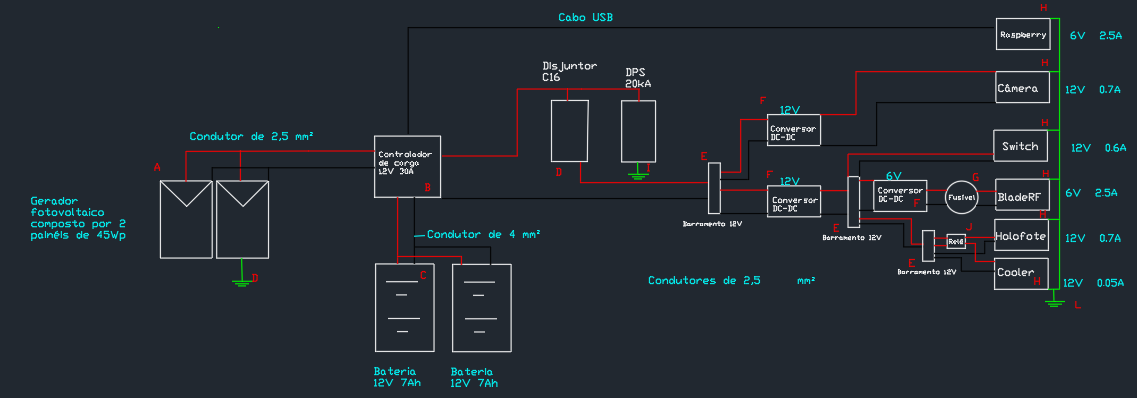
\includegraphics[scale=0.5]{df}
\caption{Diagrama unifilar - AutoCad}
\label{fig:5}
\end{figure}

Legenda:

Em “A” representa os geradores fotovoltaicos ligados em paralelo, que irão gerar em corrente alternada para alimentar a carga. Antes irá passar pelo controlador de carga “B” que irá alimentar a bateria “C” que irá alimentar a carga. Antes de chegar definitivamente na carga irá passar pelos conversores DC-DC Step-Up “E” e Step-Down “F” que irá deixar a tensão no nível na qual a carga necessita. Em seguida irá alimentar as cargas “H”, antes do holofote irá ter um relé “G” que irá aciona-lo apenas quando necessário.

\subsection{Custos}

\begin{itemize}
    \item \textbf{Funcionamento do radar durante 24 horas por dia}
\end{itemize}

\begin{table}[H]
\begin{tabular}{|c|c|c|c|c|}
\hline
\multicolumn{5}{|c|}{Energia}                                                 \\ \hline
Material             & Preço         & Quantidade & Total         & Marca     \\ \hline
Painel Fotovoltaico  & R\$ 395,00  & 1          & R\$ 395,00  & UP SOLAR    \\ \hline
Bateria 70Ah             & R\$ 269,99  & 1          & R\$ 269,00  & Heliar  \\ \hline
Bateria 185Ah             & R\$ 1109,99  & 1          & R\$ 1109,99  & Heliar  \\ \hline
Controlador de Carga & R\$ 49,99  & 1          & R\$ 49,90  & charge controller \\ \hline
Lâmpada de LED       & R\$ 46,00 & 1          & R\$ 46,00 & PXT         \\ \hline
Conversor DC-DC       & R\$ 15,90 & 4          & R\$ 63,90 & Tenstar Robot         \\ \hline
Relé       & R\$ 9,90 & 1          & R\$ 9,90 & Eletrogate         \\ \hline
Total & - & - & 1943,69 & - \\ \hline
\end{tabular}
\end{table}



\begin{itemize}
    \item \textbf{Funcionamento do radar durante 6 horas por dia}
\end{itemize}
\begin{table}[H]
\begin{tabular}{|c|c|c|c|c|}
\hline
\multicolumn{5}{|c|}{Energia}                                                 \\ \hline
Material             & Preço         & Quantidade & Total         & Marca     \\ \hline
Painel Fotovoltaico  & R\$ 395,00  & 1          & R\$ 395,00  & UP SOLAR    \\ \hline
Bateria 70Ah              & R\$ 269,99  & 1          & R\$ 269,00  & Heliar  \\ \hline
Controlador de Carga & R\$ 49,99  & 1          & R\$ 49,90  & charge controller \\ \hline
Lâmpada de LED       & R\$ 46,00 & 1          & R\$ 46,00 & PXT         \\ \hline
Conversor DC-DC       & R\$ 15,90 & 4          & R\$ 63,90 & Tenstar Robot         \\ \hline
Relé       & R\$ 9,90 & 1          & R\$ 9,90 & Eletrogate         \\ \hline
Total & - & - & 833,70 & - \\ \hline
\end{tabular}
\end{table}
\vspace*{\fill}
\pagebreak